\pdfoutput=1
\documentclass[10pt]{beamer}

%STANDARD PREAMBLE
%https://tex.stackexchange.com/questions/68821/is-it-possible-to-create-a-latex-preamble-header
\usepackage{../../rsrc/beamer_preamble}

%% ALLOW FOR ITEMIZE ENVIRONMENTS WITH NO PRECEDING
% SPACING, IF DESIRED
% Reference: https://tex.stackexchange.com/questions/86054/how-to-remove-the-whitespace-before-itemize-enumerate
%\usepackage{enumitem}% http://ctan.org/pkg/enumitem 
\usepackage{paralist}

% RANDOM VARIABLE
\newcommand{\x}{X}
\newcommand{\y}{Y}



%%% SIMPLE TEXT
\renewcommand{\bf}[1]{\textbf{{#1}}}
\renewcommand{\it}[1]{\textit{{#1}}}


%%% SIMPLE BIGG PARENTHESES AND BRACKETS
\newcommand{\bp}[1]{\bigg(  {#1} \bigg)}
\newcommand{\bb}[1]{\bigg[  {#1} \bigg]}

\title{Maximum Likelihood Approaches}

\begin{document}

\maketitle

\begin{frame}{Table of contents}
  \setbeamertemplate{section in toc}[sections numbered]
  \tableofcontents[hideallsubsections]
\end{frame}

%%%%%%%%%%%%
\section{Maximum Likelihood}

\begin{frame}{Parametric Models \hfill \tiny (apologies to Peter Orbanz) }

\begin{sblock}{Models}
A \bf{model} $\mathcal{P}$ is a set of probability distributions.  We index each distribution with a parameter value $\theta \in \Theta$; we can then write the model as
\[ \mathcal{P} = \set{P_\theta \cond \theta \in \Theta} \]
The set $\Theta$ is called the \bf{parameter space} of the model.
\end{sblock}

\begin{sblock}{Parametric model}
The model is called \bf{parametric} if the number of parameters (i.e. the vector $\theta$) is (1) finite and (2) independent of the number of data points.   Intuitively, the complexity of a parametric model does not increase with sample size.
\end{sblock}


\begin{sblock}{Density representation}
For parametric models, we can assume that $\Theta \subset \R^d$ for some fixed dimension $d$.   We usually represent each $P_\theta$ via a density function $p(x \cond \theta)$.
\end{sblock}
\hfill \tiny Slides in this section heavily borrow from Peter Orbanz.
\end{frame}


%%%%%%%%%%%%%%%%
\begin{frame}{Maximum Likelihood Estimation}
\begin{sblock}{Setting}
\begin{itemize}
\item Given: Data $x_1, ..., x_n$, parametric model $\mathcal{P} = \set{P_\theta \cond \theta \in \Theta}$
\item Objective: Find the distribution in $\mathcal{P}$ which best explain the data.  That means we have to choose a ``best" parameter value $\widehat{\theta}$.
\end{itemize}
\end{sblock}

\begin{sblock}{Maximum Likelihood approach}
Maximim Likelihood assumes that the data is best explained by the distribution in $\mathcal{P}$ under which it has the highest probability (or highest density value).

Hence, the \bf{maximum likelihood estimator} is defined as
\[ \widehat{\theta}_{\text{ML}} := \argmax_{\theta \in \Theta} p(x_1, ..., x_n \cond \theta) \]
the parameter which maximizes the joint density of the data.
\end{sblock}

\end{frame}


%%%%%%%%%%%%%%%%
\begin{frame}{The i.i.d. assumption}

\begin{sblock}{The i.i.d. assumption}
The standard assumption of ML methods is that the data is \bf{independent and identically distributed (i.i.d.)}, that is, generated by independently sampling repeatedly from the same distribution $\mathcal{P}$. 

If the density of $\mathcal{P}$ is $p(x \cond \theta)$, that means the joint density decomposes as 
\[  p(x_1, ..., x_n) = \ds\prod_{i=1}^n p(x_1 \cond \theta) \]
\end{sblock}

\end{frame}
%SAY: Often easiest.  Give example with Poisson.  Scipy doesn't support a fit function for discrete random variables.   Statsmodels library requires specification of an "exog" variable (used for nothing), the returned parameter is nested in a table of way too much information, and if you can find it, it needs to be exponentiated. 

\begin{frame}{Illustration}
\begin{center}
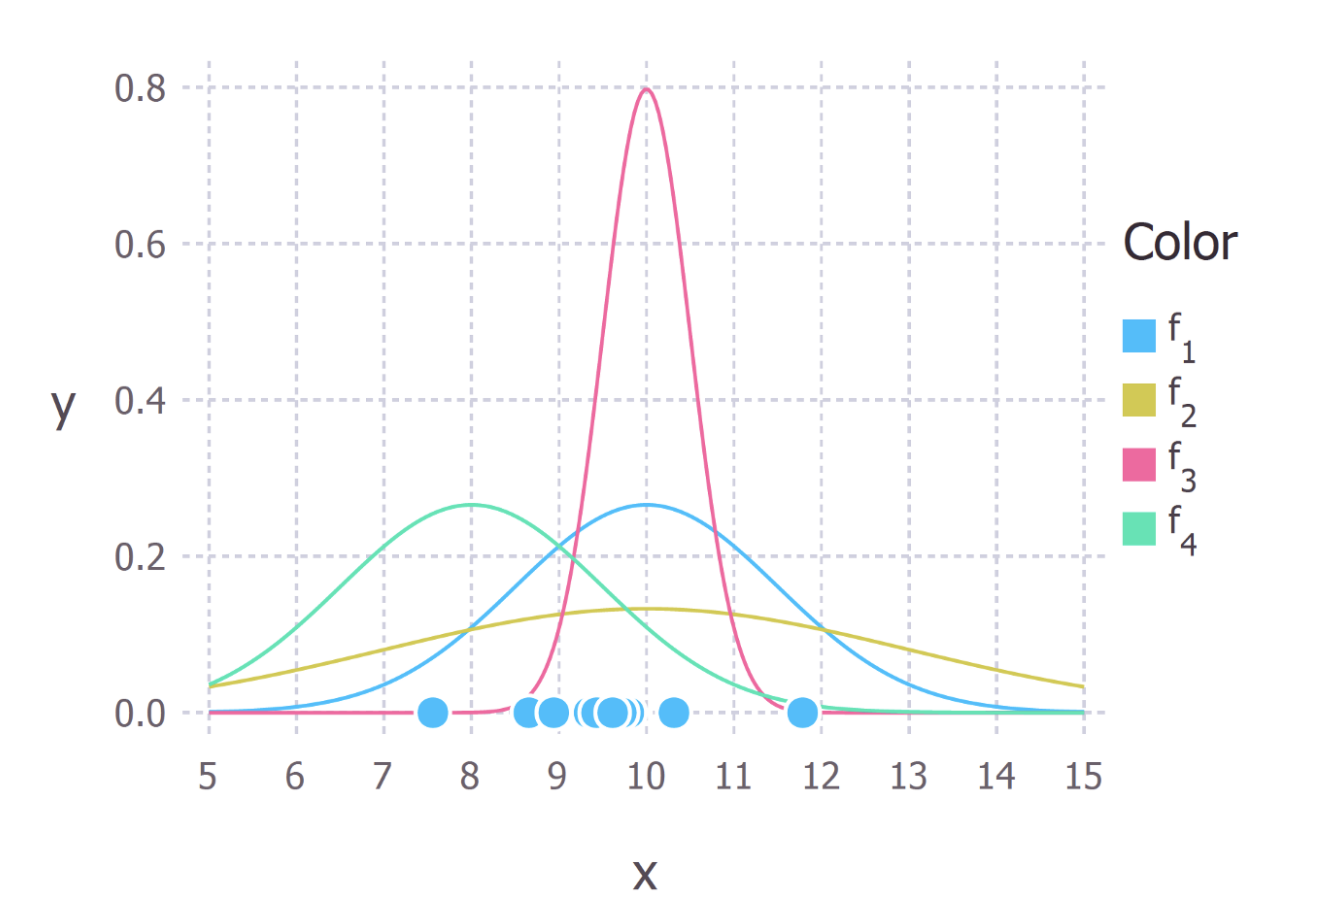
\includegraphics[width=.8\textwidth]{images/ml_example}

\vfill
\scriptsize Ten data points and four possible Gaussians from which they were drawn: $f_1 \sim \mathcal{N}(10, 2.25), f_2 \sim \mathcal{N}(10, 9), f_3 \sim \mathcal{N}(10, 0.25), f_4 \sim \mathcal{N}(8, 2.25)$.   \\ %Which distribution is the most likely to have generated the data points?
\end{center}
\hfill \tiny Image Credit: Jonny Brooks-Bartlett
% Reference https://towardsdatascience.com/probability-concepts-explained-maximum-likelihood-estimation-c7b4342fdbb1
\end{frame}


\begin{frame}{Analytic Maximum Likelihood}
\begin{sblock}{Maximum Likelihood equation}
The analytic criterion for a maximum likelihood estimator (under the i.i.d assumption) is 
\[ \nabla_\theta \bigg( \ds\prod_{i=1}^n p(x_i \cond \theta) \bigg) =0  \]
\end{sblock}
We use the ``logarithm trick" to avoid a huge product rule computation.
\end{frame}


\begin{frame}{Logarithm Trick}

\begin{sblock}{Recall: Logarithms turn products into sums}
\[ \log \bp{\ds\prod_i f_i} = \ds\sum_i  \log (f_i) \]
\end{sblock}

\begin{sblock}{Logarithms and maxima}
The logarithm is monotonically increasing on $\R_+$.\\

Consequence: Application of log does not change the \it{location} of a maximum or minimum:

\begin{align*}
\max_y \log (g(y)) &\neq \max_y g(y)  && \text{The \it{value} changes.} \\
\argmax_y \log (g(y)) &= \argmax_y g(y)  && \text{The \it{location} does not change.}
\end{align*}


\end{sblock}


\end{frame}


\begin{frame}{Analytic Maximum Likelihood}

\begin{sblock}{Likelihood and logarithm trick}
\[  \widehat{\theta}_{\text{ML}} = \argmax_\theta \ds\prod_{i=1}^n p(x_i | \theta) = \argmax_\theta \log \bp{ \ds\prod_{i=1}^n p(x_i | \theta)} = \argmax_\theta \ds\sum_{i=1}^n \log p(x_i | \theta)  \]
\end{sblock}

\begin{sblock}{Analytic maximality criterion}

\[ 0 = \ds\sum_{i=1}^n \nabla_\theta \log p(x_i | \theta) = \ds\sum_{i=1}^n \df{\nabla_\theta p(x_i |\theta) }{p(x_i |\theta)} \]

Whether or not we can solve this analytically depends on the choice of model!
\end{sblock}

\end{frame}




\begin{frame}{Example: Gaussian Distribution}

\begin{sblock}{Gaussian density in one dimension}
\begin{columns}
\begin{column}{.55\textwidth}
\footnotesize
\[ g(x; \mu, \sigma) := \df{1}{\sqrt{2 \pi} \sigma} \exp \bp{ - \df{(x-\mu)^2}{2 \sigma^2}} \]
\begin{compactitem}
\item $\mu$ = expected value of $x$, $\sigma^2$ = variance, $\sigma$ =  standard deviation
\item The quotient $\frac{x - \mu}{\sigma}$ measures deviation of $x$ from its expected value in units of $\sigma$ (i.e., $\sigma$ defines the length scale).
\end{compactitem}
\end{column}
\begin{column}{.3\textwidth}
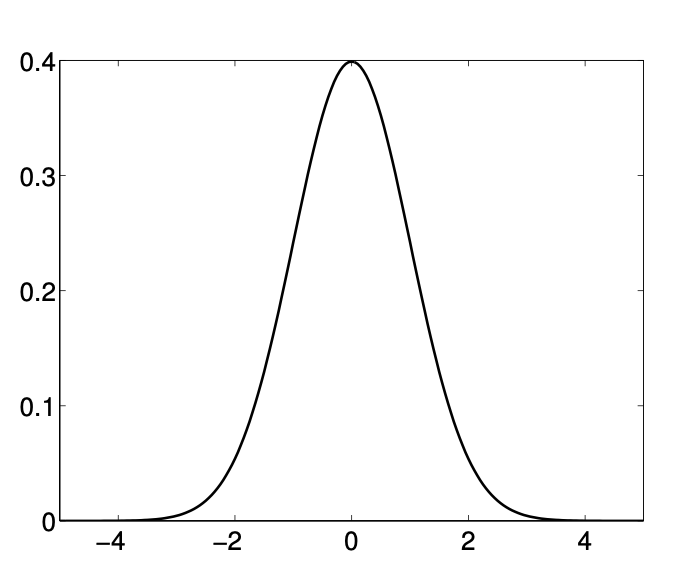
\includegraphics[width=\textwidth]{images/gaussian_1d}
\end{column}
\end{columns}
\end{sblock}

\begin{sblock}{Gaussian density in $d$ dimensions}
\begin{columns}
\begin{column}{.55\textwidth}
\footnotesize
\vfill \vfill \vfill
The quadratic function 
\[ - \df{(x-\mu)^2}{2 \sigma^2} = -\df{1}{2} (x-\mu) (\sigma^1)^{-1} (x - \mu) \]
is replaced by a quadratic form:
\[ g(\+x; \+\mu, \Sigma) := \df{1}{\sqrt{2 \pi |\Sigma|}} \exp \bp{ - \df{1}{2} (\+x - \+\mu)^T \Sigma^{-1} ( \+x - \+\mu)} \]
\end{column}
\begin{column}{.3\textwidth}
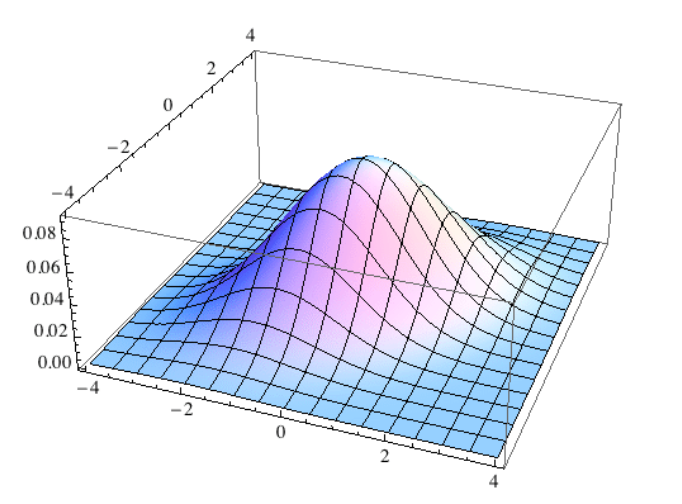
\includegraphics[width=\textwidth]{images/gaussian_nd}
\end{column}
\end{columns}
\end{sblock}

\end{frame}



\begin{frame}{Example: Gaussian Mean MLE}

\begin{sblock}{Model: Multivariate Gausians}
The model $\mathcal{P}$ is the set of all Gaussian densities on $\R^d$ with \textit{fixed} covariance matrix $\Sigma$
\[ \mathcal{P} = \set{g(\cdot \cond \mu, \Sigma) \cond \mu \in \R^d} \]
where $g$ is the Gaussian density function.  The parameter space is $\Theta = \R^d$.
\end{sblock}

\begin{sblock}{MLE equation}

We have to solve the maximum likelihood equation 
\[ \ds\sum_{i=1}^n \nabla_\mu \log g(x_i \cond \mu, \Sigma) = 0 \]
for $\mu$.
\end{sblock}

\end{frame}


\begin{frame}{Example: Gaussian Mean MLE}
\footnotesize
\begin{align*}
0 &= \ds\sum_{i=1}^n  \nabla_\mu  \log \bb{\df{1}{\sqrt{(2 \pi)^d |\Sigma| }} \exp \bp{ - \df{1}{2} (\+x - \+\mu)^T \Sigma^{-1} ( \+x - \+\mu)}}   \\
&=  \ds\sum_{i=1}^n   \nabla_\mu  \bb{\log \df{1}{\sqrt{(2 \pi)^d |\Sigma| }}} +\nabla_\mu \bb{ \log \bp{\exp \bp{ - \df{1}{2} (\+x - \+\mu)^T \Sigma^{-1} ( \+x - \+\mu)} }} \\
&=  \ds\sum_{i=1}^n \nabla_\mu \bp{ - \df{1}{2} (\+x - \+\mu)^T \Sigma^{-1} ( \+x - \+\mu)}  = -  \ds\sum_{i=1}^n \Sigma^{-1} (x_i - \+\mu) 
\end{align*}

Multiplication by $(- \Sigma)$ gives

\[  0 = \ds\sum_{i=1}^n (x_i - \+\mu) \implies \+\mu = \df{1}{n} \ds\sum_{i=1}^n x_i\]

\begin{sblock}{Conclusion}
The maximum likelihood estimator of the Gaussian expectation parameter for fixed covariance is 
\[ \widehat{\+\mu}_{\text{ML}} := \df{1}{n} \ds\sum_{i=1}^n x_i \]
\end{sblock}

\end{frame}


\begin{frame}{Example: Gaussian with Unknown Mean, Covariance}
\footnotesize
\begin{sblock}{Model: Multivariate Gaussians}
The model $\mathcal{P}$ is now
\[ \mathcal{P} = \set{g(\cdot \cond \mu, \Sigma) \cond \mu \in \R^d, \Sigma \in \Delta_d} \]
where $\Delta_d$ is the set of postive definite $d \times d$-matrices. The parameter space is $\Theta = \R^d \times \Delta_d$.
\end{sblock}

\begin{sblock}{ML approach}
Since we have just seen that the ML estimator of $\mu$ does not depend on $\Sigma$, we can compute $\widehat{\+\mu}_\text{ML}$ first. We then estimate $\Sigma$ using the criterion

\[ \ds\sum_{i=1}^n \nabla_\Sigma \log g(x_i \cond \widehat{\+\mu}_\text{ML}, \Sigma) = 0 \]
for $\mu$.
\end{sblock}

\begin{sblock}{Solution}
The ML estimator of $\Sigma$ is 

\[  \widehat{\Sigma}_\text{ML} = \df{1}{n} \ds\sum_{i=1}^n (x_i -  \widehat{\mu}_\text{ML}) (x_i - \widehat{\mu}_\text{ML})^T \]
for $\mu$.
\end{sblock}

\end{frame}



\section{Anomaly Detection}

\begin{frame}{Anomaly Detection with Multivariate Gaussians}

Given a fitted Gaussian model, how can we assess the anomalousness of test data?

\pause 
\begin{center}
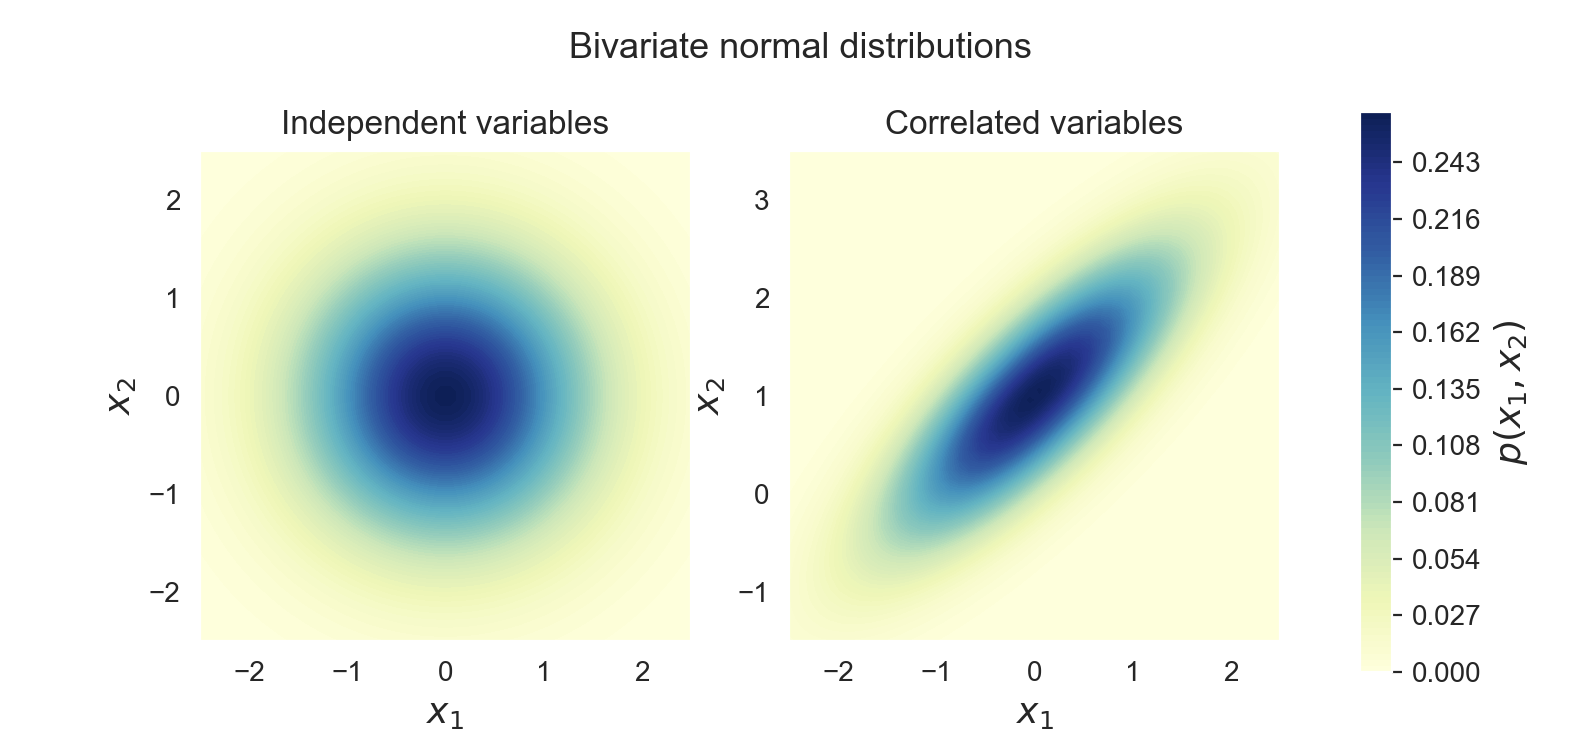
\includegraphics[width=.6\textwidth]{images/gaussian_heatmap_independent_correlated}
\end{center}

\vfill
\hfill \tiny Image Credit: Peter Roelants
\pause

\begin{sblock}{Mahalanobis Distance}
\footnotesize
For a Gaussian random variable $X \sim N (\+\mu, \Sigma)$,  the quadratic form (or \it{squared Mahalanobis distance}) has known distribution 

\[ \Delta^2 = (\+X - \+\mu) ^T \Sigma^{-1} (\+X - \+\mu) \sim \chi^2(d) \]

This can be used to assess the anomalousness of test data.
\end{sblock}
% SAY:  Note from the density that these are equi-probability contours 

\end{frame}





\end{document}